\documentclass[a4paper, reqno, 12pt, openbib]{article} % document class amsart class, draft points out the lines that are two long, reqno puts equations numbers to the right
\usepackage{geometry}\geometry{a4paper,total={170mm,250mm},left=20mm,top=25mm} % define margins of the document
\usepackage{graphicx} % package to load illustrations
\usepackage{listings} % package to read a programming language if included
\usepackage{float} % package needed to fix figures in place
\usepackage[utf8]{inputenc}
\usepackage[english]{babel}
\usepackage{amssymb}
\usepackage{amsmath}
\usepackage{color} 
\usepackage{hyperref} % enable hyperlinks in the document 
\hypersetup{
    colorlinks = true,
    linktoc = all,
    citecolor=green,
    filecolor=black,
    linkcolor=blue,
    urlcolor=red
}
% --------------------------- PREAMBLE --------------------------------------------%
\begin{document}
\title{Non-linear mechanics notes}
\author{Pradeep Janakiraman \thanks{TU Delft student from 2019-2021, notes written in Quarter 2 of AY 2020-2021}\\
3ME department\\
TU Delft, The Netherlands\\
pradeepjanakiraman@student.tudelft.nl}
\date{9 November 2020}
\maketitle
%---------------------------- TITLE PAGE ------------------------------------------%
\newpage
\tableofcontents
\newpage
%-----------
\section{Introductory material about the course}
The preknowlege required for this course are advanced dynamics (mechanics of machines), continuum mechanics (mechanics of materials) and mathematics from undergraduate courses. Resources for this course include a reader on the brightspace portal, lecture slides and recommended reading from textbooks. These notes are made during the lecture for additional reinforcement and absorption of the material.\\
\newline 
The lecture format is usally a one hour traditional lecture followed by a short break and an online test to revise the material that was covered. Every week, there is a question hour where techincal questions can be asked. The assesment for this course is one final exam, that is likely to be held online due to COVID-19. 
\section{Lecture 1}
Examples of non-linear behaviour: 
\begin{itemize}
	\item Vibration of guitar strings 
	\item Thin-walled vessel 
	\item Biological examples: Brain growth shape arising from non-linear compression. 
\end{itemize}
There are two types of non-linear behaviour \emph{Geometrically non-linear} and \emph{Physically non-linear}. Consider the pure rotation of a disc below for an example of a simple case of geometric non-linearity. 
\begin{figure}[H]
	\centering 
	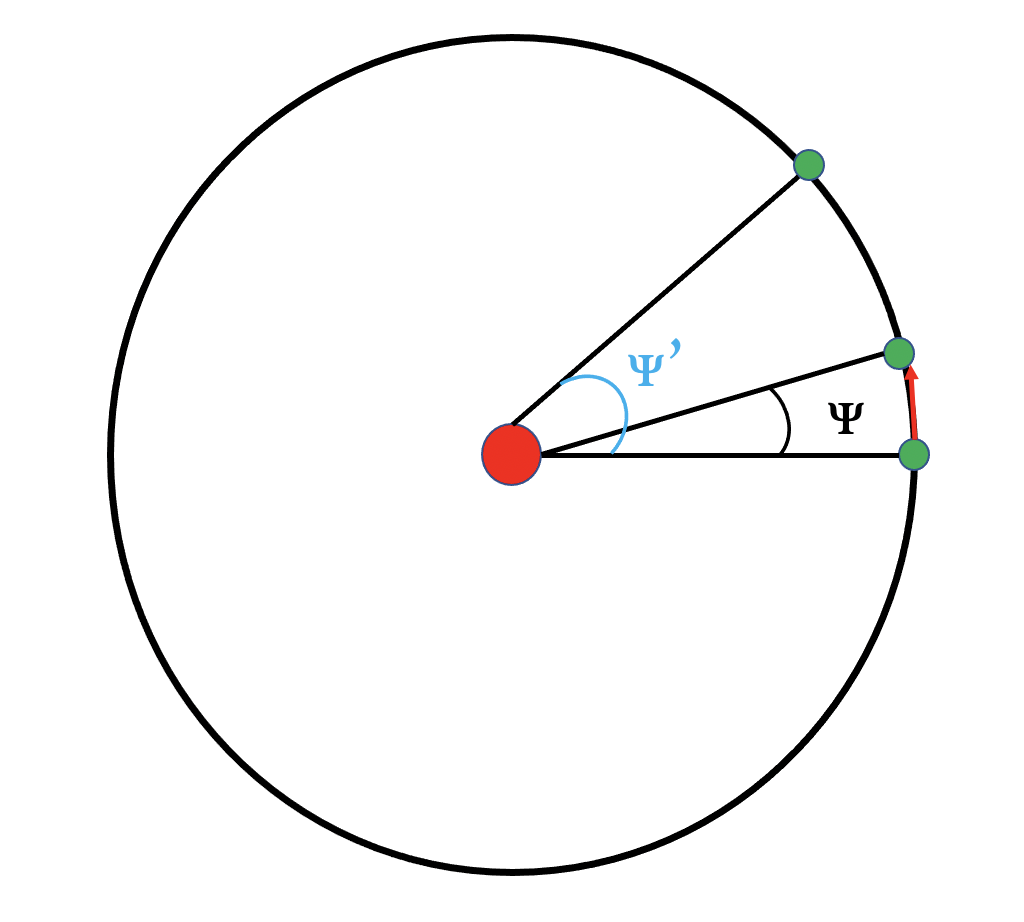
\includegraphics[scale = 0.4]{Lecture 1_nlm/images/Geometric nl}
	\caption{Example of geoemtric non-linearity}
	\label{geometric non-linearity}
\end{figure}
For small angles, 
\begin{equation}
	s = R \psi
	\label{small angle formula}
\end{equation}

But if we use the same relation for large angles, we have the case where the radius of the disc seems to be increasing, which is not correct. Physically non-linearly refers to deformations of solid objects. 
\subsection{Continuum theory}
When we consider the physical processes that happen on a piece of material, the lenght scales involved in the process have to considered. Each physical material has an internal microstructure of a certain lenght scale (for example, a sponge maybe has a microstructure $\approx 1mm$. While a piece of metal might have a microstructure $<< 1mm$). If we are interested in fluctuations that are at same order of maginitude as the microstructure, continuum theory \emph{does not apply}. In statics therefore, we only consider fluctuations that are at a much larger in magnitude that the lenght scales of the internal microstructure.\\
\newline
In mechanics, we are usually given the external load on a deformable system. From these loads we then try to find the stresses on the matrial which can be used to find the deformations and displacements. The course will first focus on the realtionship between displacements and deformations. Before moving onto the external loads and stresses. 
\subsection{Principle of virtual work} 
If we solve for the kinematics of the system, we can use the principle of virtual work to arrive at the equilibirum equations. The method is attractive due to the fact that the mathematics seem to take care of constraints and the reaction forces that arise from the constraints. From the figure below, we can see an example of the principle of virtual work at play. 
% insert figure of torisional spring and bar
\begin{figure}[H]
	\centering 
	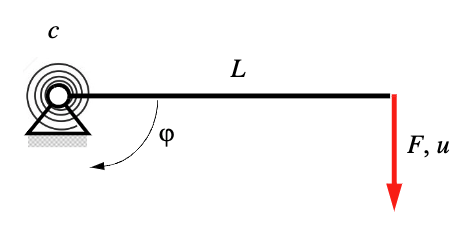
\includegraphics[scale = 0.6]{Lecture 1_nlm/images/virtual disp}
	\caption{Example of applying principle of virtual work}
	\label{egs virtual work}
\end{figure}
The kinematics of the bar with $\phi$ as a generalised coordinate: 
\begin{equation}
	u = L\sin \phi
	\label{kinematics 1dof bar}
\end{equation}
The principle of virutal displacement then requires that, 
\begin{align}
	\delta W_{internal} &= \delta W_{external}\\
	M\delta \phi &= F \delta u
\end{align}
Substituting the value of $\delta u$ from \autoref{kinematics 1dof bar}. 
\begin{align}
	M &= FL\cos \phi\\
	c \phi &= FL\cos \phi
\end{align}
The equation for the 1dof bar is therefore clearly a non-linear equation. 
























\end{document}